\documentclass[tikz,border=2pt]{standalone}

\usepackage{graphicx}
\usepackage{tikz}
\usetikzlibrary{arrows.meta, positioning, fit, backgrounds}

\begin{document}
\begin{tikzpicture}[
    font=\sffamily\small,
    >=Stealth,
    block/.style={draw, align=center, minimum height=1.0cm, rounded corners=3pt, fill=white, inner sep=5pt},
    cblock/.style={draw, align=center, minimum height=1.25cm, rounded corners=3pt, fill=gray!8, inner sep=6pt, very thick},
    img/.style={inner sep=0pt, align=center},
    op/.style={circle, draw, fill=white, inner sep=1.5pt, font=\large, minimum size=0.55cm},
    arrow/.style={->, thick},
    softarrow/.style={->, thick, gray!75},
    panel/.style={draw=black, rounded corners=5pt, inner sep=0.45cm, fill=gray!3},
]
\def\topw{1.65cm}
\def\detailw{1.45cm}

% Top-level pipeline
\node[img] (aTop) at (-4.6, 2.8) {
\includegraphics[width=\topw]{../../figures/darcy/darcy_flux_a.png}};
\node[below=2pt of aTop, font=\bfseries] {$a$};

\node[block, right=0.95cm of aTop, text width=2.0cm, font=\bfseries] (bbTop) {Backbone};
\draw[arrow] (aTop) -- (bbTop);

\node[img, right=0.95cm of bbTop] (psiTop) {
\includegraphics[width=\topw]{../../figures/darcy/darcy_flux_psi.png}};
\node[below=2pt of psiTop, font=\bfseries] {$\psi$};
\draw[arrow] (bbTop) -- (psiTop);

\node[cblock, right=1.0cm of psiTop, text width=2.35cm, font=\bfseries] (constraintTop) {Flux\\constraint};
\draw[arrow] (psiTop) -- (constraintTop);

\node[img, right=1.0cm of constraintTop] (uTop) {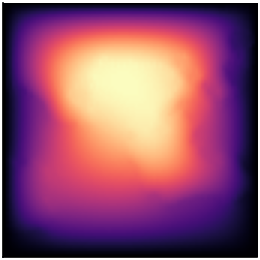
\includegraphics[width=\topw]{../../figures/darcy/darcy_flux_u.png}};
\node[below=2pt of uTop, align=center, font=\footnotesize] {$u$};
\draw[arrow] (constraintTop) -- (uTop);

% Expanded constraint block
\node[font=\bfseries] (psiOut) at (-7.0, -0.5) {$\psi$};

\node[block, right=0.8cm of psiOut, text width=1.0cm] (curl) {$\nabla^\perp$};
\draw[arrow] (psiOut) -- (curl);

\node[img, right=0.7cm of curl] (vcorr) {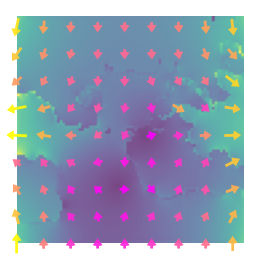
\includegraphics[width=\detailw]{../../figures/darcy/darcy_flux_vcorr.png}};
\node[below=2pt of vcorr, align=center, font=\footnotesize] {$\mathbf{v}_{\mathrm{corr}}$\\$\nabla\!\cdot\!\mathbf{v}=0$};
\draw[arrow] (curl) -- (vcorr);

\node[op, right=0.75cm of vcorr] (sum) {$+$};
\draw[arrow] (vcorr) -- (sum);

\node[img, right=0.75cm of sum] (vvalid) {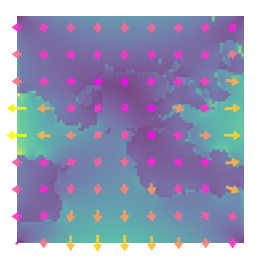
\includegraphics[width=\detailw]{../../figures/darcy/darcy_flux_vvalid.png}};
\node[below=2pt of vvalid, align=center, font=\footnotesize] {$\mathbf{v}_{\mathrm{valid}}$\\$\nabla\!\cdot\!\mathbf{v}=1$};
\draw[arrow] (sum) -- (vvalid);

\node[block, right=0.7cm of vvalid, text width=2.1cm] (law) {Darcy law\\$\mathbf{w}=-\mathbf{v}_{\mathrm{valid}}/a$};
\draw[arrow] (vvalid) -- (law);

\node[img, right=0.7cm of law] (w) {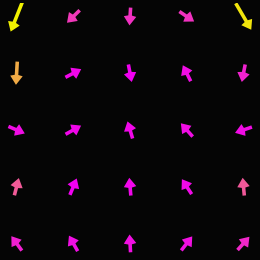
\includegraphics[width=\detailw]{../../figures/darcy/darcy_flux_w.png}};
\node[below=2pt of w, align=center, font=\footnotesize] {$\nabla u$};
\draw[arrow] (law) -- (w);

\node[block, right=0.7cm of w, text width=2.0cm] (solve) {Dirichlet sine\\Poisson solve};
\draw[arrow] (w) -- (solve);

\node[font=\bfseries, right=0.8cm of solve] (uOut) {$u$};
\draw[arrow] (solve) -- (uOut);

\node[img, below=1.5cm of sum] (vpart) {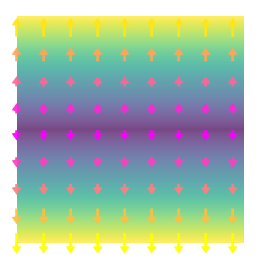
\includegraphics[width=\detailw]{../../figures/darcy/darcy_flux_vpart.png}};
\node[below=2pt of vpart, align=center, font=\footnotesize] (vpartCaption) {$\mathbf{v}_{\mathrm{part}}$\\fixed, $\nabla\!\cdot\!\mathbf{v}=1$};
\draw[arrow] (vpart) -- (sum);

\node[img, below=1.1cm of law] (aDetail) {
\includegraphics[width=\detailw]{../../figures/darcy/darcy_flux_a.png}};
\node[below=2pt of aDetail, font=\footnotesize] {$a$};
\draw[arrow] (aDetail) -- (law);

\begin{scope}[on background layer]
    \node[panel, fit=(curl)(vcorr)(sum)(vvalid)(law)(w)(solve)(vpart)(vpartCaption)(aDetail)] (expandedPanel) {};
\end{scope}
\draw[softarrow, dashed] (constraintTop.south west) -- (expandedPanel.north west);
\draw[softarrow, dashed] (constraintTop.south east) -- (expandedPanel.north east);

\end{tikzpicture}
\end{document}
